観測データ$\dv$と理論モデル$\fv$との比較により以下のようなことが得られる。
\begin{enumerate}
\item ある理論モデル$\fv$は観測データを説明できるモデルかどうか知る 
\item ある理論モデル$\fv$が正しいとしたとき、そのモデル内に含まれるパラメタ$\thetav$をデータ$\dv$にもとづいて決定・推定する ({\bf パラメタ推定})
\item 複数のモデルが存在するときにどちらのモデルが観測$\dv$をよく説明できるか ({\bf モデル選択})
\end{enumerate}
モデル選択はいろいろ大変なので、ここではパラメタ推定について考える。



ここでは例として以下にあげる視線速度の観測データと理論モデルの比較を行う。この場合、$\dv$はrvデータ列を並べたベクトルと考えればよく、各要素$d_i$はこれに対応する時間$t_i$を通じて、理論モデルと比較可能となる。理論モデルは式(\ref{eq:vrsatarefinal})である。パラメタベクトルは$\thetav = (V_\mathrm{sys}, K_\star, e, \omega, T_0, P)$であることがわかる。

\begin{itembox}{視線速度の生データ $\dv$}
\footnotesize
\color{gray}
\href{https://github.com/HajimeKawahara/class25}{https://github.com/HajimeKawahara/class25}
を参照
\end{itembox}


\section{点推定と最適化}
パラメタ$\thetav$を内部に持つモデル$\fv(\thetav)$とデータ $\dv$を何らかの手段で比較することで、一つのパラメタを選択するるパラメタ推定を\underline{点推定}という。もし、データに誤差が全く含まれていなかったら
\begin{align}
    \dv - \fv(\thetav) = \boldsymbol{0}
\end{align}
となる$\thetav$を探せばよいだろう。しかし、通常、データには観測誤差が含まれていて、このような式を満たす$\thetav$は通常見つからない。すなわち
\begin{align}
    \dv = \fv(\thetav^\ast) + \epsilonv
\end{align}
のようにかける。この式は、モデル$\fv$が正しく、かつ"正しい"パラメタ$\theta^\ast$が存在し、残差ベクトル$\epsilonv$が観測誤差のみに由来しているということを含意している。観測誤差を扱う形で理論構成を行うには、観測誤差を生成する確率モデルが必要であることがわかる。たとえば、$\epsilonv$が独立のゼロ平均の正規分布に従うとき、
\begin{align}
 \epsilon_i \sim \mathcal{N}(0,\sigma) 
\end{align}
とかける。もしくはもっと簡潔に物理モデル$\fv(\thetav^\ast)$は確率モデルの平均値であるとして
\begin{align}
    d_i \sim \mathcal{N} (f_i(\thetav^\ast), \sigma)
\end{align}
という理論モデル構成を行うことができる。

さてこの議論でわかるのは、観測データと理論モデルを比較する、といったときの理論モデルとは、$\fv$だけではなく確率モデルも指定しないとならない。図式的に書くと
\begin{itembox}{実証可能な理論モデル}
 実証可能な理論 = 物理・化学モデル + 確率モデル
\end{itembox}

通常、理論天文学では物理・化学モデルを重視しすぎるあまり確率モデルをおろそかにしがちである。また観測天文学では物理・化学モデルを固定しがちである。確率モデルの構成は、実際的な問題として計算量が多く、近年までは簡単には扱えなかった。しかし、最近は計算機の進歩とベイズ統計手法の進歩でこれに対処できるようになってきた。

さて、点推定に戻る。データ間の相関誤差がある場合も多いが、これはガウス過程によるモデリングに譲るとして、今は独立に誤差が入っているとしよう。さらにその誤差がどのデータ点に対しても同じ$\sigma$のガウシアンだとする。この場合、$\thetav$をもつモデル$\fv(\thetav)$が$\dv$を生じさせる確率は
\begin{align}
    p(\dv|\thetav) &= \prod_{i=1}^N \mathcal{N} (f_i(\thetav), \sigma ) \\
    &\propto \exp{\left( - \dfrac{\sum_{i=1}^N (f_i(\thetav) - d_i)^2 }{2 \sigma^2}\right)}
\end{align}
となる。これは尤度関数(likelihood)である。尤度を最も大きくする$\thetav$を点推定値として採用する方法を最尤法という。この場合、
\begin{align}
    \thetav^\ast &= \mathrm{minimize}_{\thetav} \, L_2(\thetav) \\
    L_2(\thetav) &= \sum_{i=1}^N (f_i(\thetav) - d_i)^2 
\end{align}
という最適化問題をとけばよいということになる。
これは最小二乗法そのものである。すなわち最小二乗法は、誤差が独立なガウシアンであると仮定したときの最尤推定と一致する。


最小二乗法による点推定の仮定をもう少しゆるくしたものが、$\chi^2$最小化である。これは、各データ点の$\sigma_i$が既知だとして
\begin{align}
    p(\dv|\thetav) &\propto \exp{\left( - \sum_{i=1}^N \dfrac{ (f_i(\thetav) - d_i)^2 }{2 \sigma_i^2}\right)}
\end{align}
となることより、
\begin{align}
    \thetav^\ast &= \mathrm{minimize}_{\thetav} \, \chi^2(\thetav) \\
    \chi^2(\thetav) &= \sum_{i=1}^N \dfrac{ (f_i(\thetav) - d_i)^2 }{2 \sigma_i^2}
\end{align}
の最適化問題を解くというものである。

\section{最適化問題と自動微分}
さてここまでの議論から、点推定の実際的な問題系は最適化問題であるということがわかる。非線形モデルの最適化問題をとくには、以前見た二次最適化としてのNewton法や、その発展である準ニュートン法、諸先生方がNumerical Recipesを熟読しながら実装したマルカート法、もしくはアメーバー法としてしられる勾配を用いないNelder-Mead法など多種多様な方法がある。

しかしここでは、自動微分を用いた一次の最適化を考える。これはパラメタ数が多いと二次最適化はヘッシアン計算に律速されるためである。そのためニューラルネットなどの機械学習モデルは一次最適化を用いることが多い。一次最適化の基本は最急降下法であり
\begin{eqnarray}
\thetav^{(k)} &=& \displaystyle{\thetav^{(k-1)} - \gamma \frac{\partial}{\partial \thetav} f(\thetav)}
\end{eqnarray}
のように、最も急な坂を下っていく方法である。最急降下法だと行き過ぎることがおおいので、さまざまなモーメントをつけて落ちやすくする。代表的な方法はADAM\cite{kingma2015adam}であるがここではアルゴリズムの詳細には踏み入れない。

\begin{figure}[htb]
\begin{center}
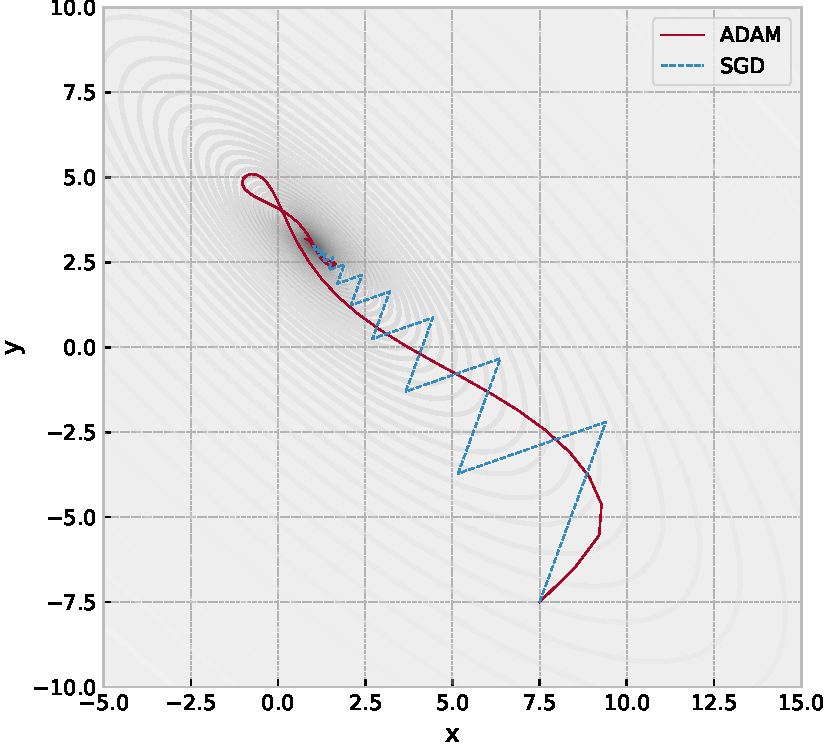
\includegraphics[width=\linewidth]{fig/opt1.pdf}
\caption{一次最適化の例。\label{fig:opt1}}
\end{center}
\end{figure}

一次最適化では、モデルのパラメタによる微分が必要である。数値的に微分値を求めるにはおおまかに4つの方法がある。一つ目は手で微分(manual differentiation)をし、結果をコーディングすることである。これはモデルが複雑になってくると破綻しがちであり、またフレキシビリティの観点からもモデルの継続的な改良を妨げる。次にmathematica等によるsymbolic differentiationを用いて手で微分する代わりに微分結果を得てコーディングすることが考えられる。これはmathematica等を用いたことのある方ならばわかると思うが、モデルが複雑になってくると膨大な項数の結果が排出されるので、やはりフレキシビリティの観点からは難点がある。次に、数値微分を行うことが考えられる。数値微分はモデルが複雑になってくるとエラーがたまりやすい。そこで機械学習分野などで用いられているのが{\sf JAX}/tensorflow/pytorchなどで用いられている、自動微分である。コーディングできるモデルは通常、様々な微分の既知である関数(ここでは要素関数と呼ぼう)の加減乗除の組み合わせでできている。そこで、自動微分では、連鎖則が成り立つように各要素関数
\begin{eqnarray}
x:\to f(x)
\end{eqnarray}
を関数のアウトプットとその微分値の情報
を出力するように拡張する。また微分の加乗除の演算規則がなりたつように演算を定義する。自動微分の実装法としては{\sf JAX}ではJacovian Vector Product (JVP)を用いたものが使用されている。しかしここではイントロダクションとしてより説明が容易な、双対数を用いた方式を使用して自動微分を解説しよう。

双対数(dual number)、$z \in k[\epsilon]/\langle \epsilon^2\rangle$\footnote{多項式環の商環のことをしめしている。詳しくはたとえば雪江明彦「環と体とガロア理論」などを参照。}は$a, b \in \mathbb{R}$にたいし、
\begin{eqnarray}
z &=& a + b \epsilon \\
\epsilon^2 &=& 0
\end{eqnarray}
となる数である。複素数は$i^2 = -1$であったのが$\epsilon^2 = 0$となったと考えればよい。変数$x$の拡張として実部$a$に$x$を、非実部$b$に$x^\prime$を割り当てると、$z = f + f^\prime \epsilon, w = g + g^\prime \epsilon$に対し、可算・乗数・除算はそれぞれ
\begin{eqnarray}
\label{eq:add_ad_dual}
z + w &=& (f + g) + (f^\prime + g^\prime) \epsilon \\ 
\label{eq:mul_ad_dual}
z w &=& f g + (f^\prime g + f g^\prime) \epsilon\\ 
z/w &=& \frac{f}{g} + \frac{f^\prime g - f g^\prime}{g^2} \epsilon
\end{eqnarray}
となる。これは実部に関して通常の、また非実部に関して微分の加乗除則と同じであることを示している。次に連鎖則を実現するには関数$x:\to F(x)$を
\begin{eqnarray}
\label{eq:funcdual}
x+x^\prime \epsilon: \to F(x) + F^\prime(x) x^\prime \epsilon  
\end{eqnarray}
と拡張すればよい。ここで$F(x)$を元の関数、双対数をもつ拡張された関数を$\hat{F}(x+x^\prime \epsilon)$と分けて表記する。すると式(\ref{eq:funcdual})は
\begin{eqnarray}
\label{eq:chain_ad}
\hat{F}(x+x^\prime \epsilon) =  F(x) + F^\prime(x) x^\prime \epsilon
\end{eqnarray}
と書ける。さて連鎖則$G(F(x))$の拡張は
\begin{eqnarray}
\hat{G}(\hat{F}(x+x^\prime \epsilon)) &=&  \hat{G}(F(x) + F^\prime(x) x^\prime \epsilon) \\
&=& G(F(x)) + G^\prime(F(x)) F^\prime(x) x^\prime \epsilon
\end{eqnarray}
となり、実部は通常の合成($G(F(x))$)が、非実部は連鎖則$G^\prime(F(x)) F^\prime(x) x^\prime = \frac{d G}{d F} 
\frac{d F}{d x} x^\prime$が実現されているのが確認できる。

\subsection*{ミニマム自動微分実装}
というわけで小さな自動微分をPythonで実装してみよう。ここで解きたい問題を
\begin{eqnarray}
\label{eq:sample_func}
F(x) = \log{(\cos{x} \sin{x})} + \sin{x}
\end{eqnarray}
の$x=1$で微分 $F^\prime(1)$とする。さらにその合成関数
\begin{align}
\label{eq:dualad2}
G(x) &= F(F(x))
\end{align}
の$x=1$での微分$G^\prime(1)$も求めたい。式(\ref{eq:dualad2})を手で微分するのは大変であるし、symbolic differentiationの結果も長大である。しかし自動微分ならばかなりすっきりしたコードになる。

まず関数(\ref{eq:sample_func})に存在する演算は可算と乗算であるので、式(\ref{eq:add_ad_dual})、(\ref{eq:mul_ad_dual})に対応した双対数の可乗算を定義する。
\begin{minted}[linenos=true, frame=single, numbersep=6pt, mathescape=true]{python}
def mul(x, y):
    a, b = x
    c, d = y
    return a*c, a*d + b*c

def add(x, y):
    a, b = x
    c, d = y
    return a + c, b + d
\end{minted}
ここに$x,y$はそれぞれ双対数である。次に関数(\ref{eq:sample_func})に存在する要素関数は$\sin{x}$、$\cos{x}$、$\log{x}$である。式(\ref{eq:chain_ad})を実装するには、双対数の実部と非実部をペア$(a,b)$の形式であらわすと、関数$F(x)$に対し
\begin{eqnarray}
(x,dx) \to (F(x),F^\prime(x) dx) 
\end{eqnarray}
となるように入出力を与えればよいことがわかる。そこで
\begin{minted}[linenos=true, frame=single, numbersep=6pt, mathescape=true]{python}
import numpy as np
def cos(x):
    a, b = x
    return np.cos(a), - np.sin(a)*b

def sin(x):
    a, b = x
    return np.sin(a), np.cos(a)*b
    
def log(x):
    a, b = x
    return np.log(a), b/a 
\end{minted}
これで終わりである。あとは

\begin{minted}[linenos=true, frame=single, numbersep=6pt, mathescape=true]{python}
f = lambda x: 
add(log(mul(cos(x),sin(x))),sin(x))
df = lambda x: f([x,1.0])
df(1.0)
\end{minted}
とすれば$(F(1), F^\prime(1))$が (0.05324076815279066, -0.37501280285243144)と求まる。$G^\prime(x)$も簡単で、
\begin{minted}[linenos=true, frame=single, numbersep=6pt, mathescape=true]{python}
g = lambda x: f(f(x))
dg = lambda x: g([x,1.0])
dg(1.0)
\end{minted}
とするだけで(-2.8816056725768977, -7.391555094461485)と求まる。以上の例からわかるように自動微分の実際の計算には代数計算を用いているため数値微分に比べて誤差の蓄積は少ない。またフレキシブルにコーディングが可能である。

ここでは自分で実装してみたが、実際にはJAXやpytorch, Enzyme.jlなどの自動微分パッケージを利用することになるだろう。さらに自動微分は、次に示すベイズ統計的なパラメタ推定でも威力を発する。このようにコードをエンドトゥーエンドで微分可能にしておくプログラミングを\underline{微分可能プログラミング}という\cite{2024arXiv240314606B}。